\documentclass[10pt,ignorenonframetext,,aspectratio=149]{beamer}
\usefonttheme{serif} % use mainfont rather than sansfont for slide text
\setbeamertemplate{caption}[numbered]
\setbeamertemplate{caption label separator}{: }
\setbeamercolor{caption name}{fg=normal text.fg}
\usepackage{lmodern}
\usepackage{amssymb,amsmath}
\usepackage{ifxetex,ifluatex}
\usepackage{fixltx2e} % provides \textsubscript
\ifnum 0\ifxetex 1\fi\ifluatex 1\fi=0 % if pdftex
  \usepackage[T1]{fontenc}
  \usepackage[utf8]{inputenc}
\else % if luatex or xelatex
  \ifxetex
    \usepackage{mathspec}
  \else
    \usepackage{fontspec}
  \fi
  \defaultfontfeatures{Ligatures=TeX,Scale=MatchLowercase}
  \newcommand{\euro}{€}
    \setmainfont[]{Open Sans}
\fi
% use upquote if available, for straight quotes in verbatim environments
\IfFileExists{upquote.sty}{\usepackage{upquote}}{}
% use microtype if available
\IfFileExists{microtype.sty}{%
\usepackage{microtype}
\UseMicrotypeSet[protrusion]{basicmath} % disable protrusion for tt fonts
}{}
\usepackage{graphicx,grffile}
\makeatletter
\def\maxwidth{\ifdim\Gin@nat@width>\linewidth\linewidth\else\Gin@nat@width\fi}
\def\maxheight{\ifdim\Gin@nat@height>\textheight0.8\textheight\else\Gin@nat@height\fi}
\makeatother
% Scale images if necessary, so that they will not overflow the page
% margins by default, and it is still possible to overwrite the defaults
% using explicit options in \includegraphics[width, height, ...]{}
\setkeys{Gin}{width=\maxwidth,height=\maxheight,keepaspectratio}

% Comment these out if you don't want a slide with just the
% part/section/subsection/subsubsection title:
\AtBeginPart{
  \let\insertpartnumber\relax
  \let\partname\relax
  \frame{\partpage}
}
\AtBeginSection{
  \let\insertsectionnumber\relax
  \let\sectionname\relax
  \frame{\sectionpage}
}
\AtBeginSubsection{
  \let\insertsubsectionnumber\relax
  \let\subsectionname\relax
  \frame{\subsectionpage}
}

\setlength{\emergencystretch}{3em}  % prevent overfull lines
\providecommand{\tightlist}{%
  \setlength{\itemsep}{0pt}\setlength{\parskip}{0pt}}
\setcounter{secnumdepth}{0}

\title{The Generalized Regression Model and Heteroskedasticity}
\author{Henrique Veras}
\date{}

%% Here's everything I added.
%%--------------------------

\usepackage{graphicx}
\usepackage{rotating}
%\setbeamertemplate{caption}[numbered]
\usepackage{hyperref}
\usepackage{caption}
\usepackage[normalem]{ulem}
%\mode<presentation>
\usepackage{wasysym}
%\usepackage{amsmath}


% Get rid of navigation symbols.
%-------------------------------
\setbeamertemplate{navigation symbols}{}

% Optional institute tags and titlegraphic.
% Do feel free to change the titlegraphic if you don't want it as a Markdown field.
%----------------------------------------------------------------------------------
\institute{PIMES/UFPE}

% \titlegraphic{\includegraphics[width=0.3\paperwidth]{\string~/Dropbox/teaching/clemson-academic.png}} % <-- if you want to know what this looks like without it as a Markdown field. 
% -----------------------------------------------------------------------------------------------------


% Some additional title page adjustments.
%----------------------------------------
\setbeamertemplate{title page}[empty]
%\date{}
\setbeamerfont{subtitle}{size=\small}

\setbeamercovered{transparent}

% Some optional colors. Change or add as you see fit.
%---------------------------------------------------
\definecolor{clemsonpurple}{HTML}{522D80}
 \definecolor{clemsonorange}{HTML}{F66733}
\definecolor{uiucblue}{HTML}{003C7D}
\definecolor{uiucorange}{HTML}{F47F24}


% Some optional color adjustments to Beamer. Change as you see fit.
%------------------------------------------------------------------
\setbeamercolor{frametitle}{fg=clemsonpurple,bg=white}
\setbeamercolor{title}{fg=clemsonpurple,bg=white}
\setbeamercolor{local structure}{fg=clemsonpurple}
\setbeamercolor{section in toc}{fg=clemsonpurple,bg=white}
% \setbeamercolor{subsection in toc}{fg=clemsonorange,bg=white}
\setbeamercolor{footline}{fg=clemsonpurple!50, bg=white}
\setbeamercolor{block title}{fg=clemsonorange,bg=white}


\let\Tiny=\tiny


% Sections and subsections should not get their own damn slide.
%--------------------------------------------------------------
\AtBeginPart{}
\AtBeginSection{}
\AtBeginSubsection{}
\AtBeginSubsubsection{}

% Suppress some of Markdown's weird default vertical spacing.
%------------------------------------------------------------
\setlength{\emergencystretch}{0em}  % prevent overfull lines
\setlength{\parskip}{0pt}


% Allow for those simple two-tone footlines I like. 
% Edit the colors as you see fit.
%--------------------------------------------------
\defbeamertemplate*{footline}{my footline}{%
    \ifnum\insertpagenumber=1
    \hbox{%
        \begin{beamercolorbox}[wd=\paperwidth,ht=.8ex,dp=1ex,center]{}%
      % empty environment to raise height
        \end{beamercolorbox}%
    }%
    \vskip0pt%
    \else%
        \Tiny{%
            \hfill%
		\vspace*{1pt}%
            \insertframenumber/\inserttotalframenumber \hspace*{0.1cm}%
            \newline%
            \color{clemsonpurple}{\rule{\paperwidth}{0.4mm}}\newline%
            \color{clemsonorange}{\rule{\paperwidth}{.4mm}}%
        }%
    \fi%
}

% Various cosmetic things, though I must confess I forget what exactly these do and why I included them.
%-------------------------------------------------------------------------------------------------------
\setbeamercolor{structure}{fg=blue}
\setbeamercolor{local structure}{parent=structure}
\setbeamercolor{item projected}{parent=item,use=item,fg=clemsonpurple,bg=white}
\setbeamercolor{enumerate item}{parent=item}

% Adjust some item elements. More cosmetic things.
%-------------------------------------------------
\setbeamertemplate{itemize item}{\color{clemsonpurple}$\bullet$}
\setbeamertemplate{itemize subitem}{\color{clemsonpurple}\scriptsize{$\bullet$}}
\setbeamertemplate{itemize/enumerate body end}{\vspace{.6\baselineskip}} % So I'm less inclined to use \medskip and \bigskip in Markdown.

% Automatically center images
% ---------------------------
% Note: this is for ![](image.png) images
% Use "fig.align = "center" for R chunks

\usepackage{etoolbox}

\AtBeginDocument{%
  \letcs\oig{@orig\string\includegraphics}%
  \renewcommand<>\includegraphics[2][]{%
    \only#3{%
      {\centering\oig[{#1}]{#2}\par}%
    }%
  }%
}

% I think I've moved to xelatex now. Here's some stuff for that.
% --------------------------------------------------------------
% I could customize/generalize this more but the truth is it works for my circumstances.

\ifxetex
\setbeamerfont{title}{family=\fontspec{Titillium Web}}
\setbeamerfont{frametitle}{family=\fontspec{Titillium Web}}
\usepackage[font=small,skip=0pt]{caption}
 \else
 \fi

% Okay, and begin the actual document...

\begin{document}
\frame{\titlepage}

\hypertarget{econometrics}{%
\section{Econometrics}\label{econometrics}}

\hypertarget{intro}{%
\subsection{Intro}\label{intro}}

\begin{frame}{Intro}
We now extend the multiple regression model to incorporate disturbances
that violate assumption A.4.

\vfill

But first things first: is the correct name heteros\emph{k}edasticity or
heteros\emph{c}edasticity?

\vfill
\end{frame}

\begin{frame}{Introduction}
\protect\hypertarget{introduction}{}
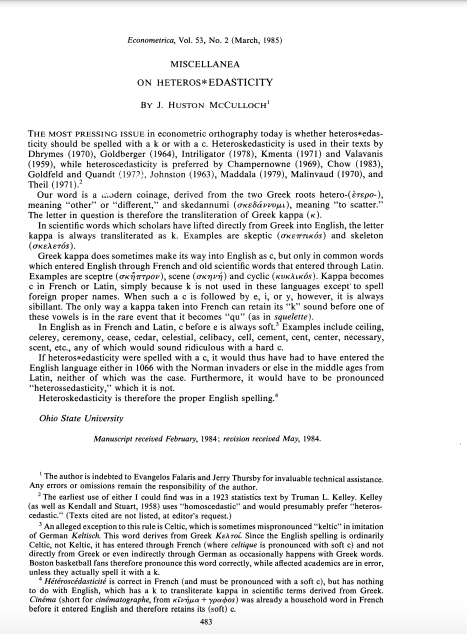
\includegraphics{econometrica.png}
\end{frame}

\begin{frame}{Introduction}
\protect\hypertarget{introduction-1}{}
The \textbf{Generalized Linear Regression Model} is

\[\begin{split}
\mathbf{y} & =  \mathbf{X\beta}+\varepsilon \\
E[\mathbf{\varepsilon}|\mathbf{X}] & =  \mathbf{0} \\
E[\mathbf{\varepsilon\varepsilon'}|\mathbf{X}] & = \sigma^2\mathbf{\Omega}=\mathbf{\Sigma} \\ \end{split}\]

where \(\Omega\) is a positive definite matrix.

\vfill

Notice that \(\sigma^2\mathbf{I}\) is a special case.

\vfill
\end{frame}

\begin{frame}{Introduction}
\protect\hypertarget{introduction-2}{}
The two leading cases are \textbf{heteroskedasticity} and
\textbf{autocorrelation}.

\vfill

Heteroskedasticity in cross-sectional data appear in data where the
scale of the dependent variable and the explanatory power of the model
tend to vary across observations.

\begin{itemize}
\tightlist
\item
  For example, we observe greater variation in expenditure on certain
  commodity groups among high-income family than in low-income ones.
\end{itemize}

\vfill

Let's focus on this issue now, still assuming that disturbances are
uncorrelated across observations.

\vfill
\end{frame}

\begin{frame}{Introduction}
\protect\hypertarget{introduction-3}{}
In the current context, \(\sigma^2\mathbf{\Omega}\) would be

\[\sigma^2\mathbf{\Omega}=\sigma^2 \begin{bmatrix}
\omega_1 & 0 & \cdots & 0 \\
0 & \omega_2 & \cdots & 0 \\
\vdots & \vdots & \ddots & \vdots \\
0 & 0 & \cdots  & \omega_n \end{bmatrix}=\begin{bmatrix}
\sigma_1^2 & 0 & \cdots & 0 \\
0 & \sigma_2^2 & \cdots & 0 \\
\vdots & \vdots & \ddots & \vdots \\
0 & 0 & \cdots  & \sigma_n^2 \end{bmatrix}\]
\end{frame}

\hypertarget{robust-least-squares-estimation-and-inference}{%
\subsection{Robust Least Squares Estimation and
Inference}\label{robust-least-squares-estimation-and-inference}}

\begin{frame}{Robust Least Squares Estimation and Inference}
The generalized model drops assumption A.4., allowing disturbances to
being heteroskedastic or autocorrelated (or both).

\vfill

The Least Squares estimator is said to be ``robust'' if it is
insensitive to departures from the base assumptions of the model.

\vfill

We can distinguish between

\begin{enumerate}
\tightlist
\item
  \textbf{Robust estimator}: A consistent estimator that remain
  consistent in spite of violations of assumpions used to motivate it.
\item
  \textbf{Robust inference}: Inference procedures are robust when they
  are based on estimators of asymptotic variances that are appropriate
  even when the assumptions are violated.
\end{enumerate}

\vfill
\end{frame}

\begin{frame}{A Heteroskedasticity-Robust Covariance Matrix for Least
Squares}
\protect\hypertarget{a-heteroskedasticity-robust-covariance-matrix-for-least-squares}{}
For the most general case, suppose
\(Var[\varepsilon_i|\mathbf{x}_i]=\sigma_i^2\)

\vfill

We can write the LS estimator as

\[\mathbf{b}=\mathbf{\beta}+(\mathbf{X'X})^{-1}\sum_{i=1}^n{\mathbf{x}_i\varepsilon_i}\]

Then,
\[Var[\mathbf{b}|\mathbf{X}]=\frac{1}{n}\left(\frac{\mathbf{X'X}}{n}\right)^{-1}\left(\frac{\mathbf{X'}(\sigma^2\mathbf{\Omega})\mathbf{X}}{n}\right)\left(\frac{\mathbf{X'X}}{n}\right)^{-1}\]

The asymptotic variance will be

\[Asy.Var[\mathbf{b}]=\frac{1}{n}\mathbf{Q}^{-1}\left[\text{plim }\frac{1}{n}\sum_{i=1}^n{\sigma_i^2\mathbf{x}_i\mathbf{x}_i'}\right]\mathbf{Q}^{-1}=\frac{1}{n}\mathbf{Q}^{-1}\mathbf{Q}^*\mathbf{Q}^{-1}\]

\vfill
\end{frame}

\begin{frame}{A Heteroskedasticity-Robust Covariance Matrix for Least
Squares}
\protect\hypertarget{a-heteroskedasticity-robust-covariance-matrix-for-least-squares-1}{}
Two points to consider:

\begin{enumerate}
\tightlist
\item
  Is \(s^2(\mathbf{X'X})^{-1}\) likely to be a valid estimator of
  \(Asy.Var[\mathbf{b}]\)?
\item
  If not, is there a strategy available that is ``robust'' to
  unspecified heteroskedasticity?
\end{enumerate}

\vfill

Based on the expression for \(Var[\mathbf{b}|\mathbf{X}]\), we see that
\(s^2(\mathbf{X'X})^{-1}\) would not be the appropriate estimator for
the asymptotic covariance matrix for the LS estimator.

\vfill

The answer to the second question is yes. What we need is a feasible
estimator of \(\mathbf{Q}^*\).

\vfill
\end{frame}

\begin{frame}{White's (1980) Heteroskedasticity-Robust Estimator}
\protect\hypertarget{whites-1980-heteroskedasticity-robust-estimator}{}
White's (1980) Heteroskedasticity-Robust Estimator of \(\mathbf{Q}^*\)
is

\[\mathbf{W}_{het}=\frac{1}{n}\sum_{i=1}^n{e_i^2\mathbf{x}_i\mathbf{x}_i'},\]

where \(e_i\) is the LS residual, \(y_i-\mathbf{x}_i'\mathbf{b}\).

\vfill

Thus, we have

\[Est.Asy.Var[\mathbf{b}]=n(\mathbf{X'X})^{-1}\mathbf{W}_{het}(\mathbf{X'X})^{-1}\]
The implication is that we can discard the homoskedasticity assumption
in A.4. and recover appropriate standard errors.

\vfill
\end{frame}

\begin{frame}{Robustness to Clustering}
\protect\hypertarget{robustness-to-clustering}{}
Settings in which the sample data consists of groups of related
observations are increasingly common:

\begin{enumerate}
\tightlist
\item
  firms grouped by industries
\item
  students in schools
\item
  homes in neighborhoods
\end{enumerate}

\vfill

Suppose that the sample consists of \(C\) groups of observations,
labeled \(c=1, \ldots, C\). There are \(N_c\) observations in group (or
cluster) \(c\), with \(c\geq1\).

\begin{itemize}
\tightlist
\item
  Thus, \(\sum_c{n}\).
\end{itemize}

\vfill
\end{frame}

\begin{frame}{Robustness to Clustering}
\protect\hypertarget{robustness-to-clustering-1}{}
The regression model is

\[y_{i,c}=\mathbf{x}_{i,c}'\mathbf{\beta}+\varepsilon_{i,c}\]

\vfill

The LS estimator is

\[\mathbf{b}=\mathbf{\beta}+\left(\sum_{c=1}^C{\mathbf{X_c'X_c}} \right)^{-1} \left[\sum_{c=1}^C{\left(\sum_{i=1}^N{\mathbf{x}_i}_{i,c}\varepsilon_{i,c} \right) } \right]=\mathbf{\beta}+(\mathbf{X'X})^{-1}\left[\sum_{c=1}^C{\mathbf{X}_c'\mathbf{\varepsilon}_c} \right]\]

where \(X_c\) is the \(N_c\times K\) matrix of exogenous variables for
cluster \(c\) and \(\mathbf{\varepsilon}_c\) is the vector of \(N_c\)
disturbances for the group.

\vfill

Here we assume that observations within a cluster are correlated but the
clusters are independent.

\vfill
\end{frame}

\begin{frame}{Robustness to Clustering}
\protect\hypertarget{robustness-to-clustering-2}{}
The variance matrix of the OLS estimator which is robust to clustering
is

\[Var[\mathbf{b}|\mathbf{X}]=(\mathbf{X'X})^{-1}\left[\sum_{c=1}^C{X_c \mathbf{\Omega}_cX_c'} \right](\mathbf{X'X})^{-1}\]

\vfill

The construction is essentially the same as in the White estimator,
though the matrix \(\mathbf{\Omega}_c\) is the matrix of variances and
covariances for the full vector \(\mathbf{\varepsilon}_c\).

\begin{itemize}
\tightlist
\item
  It would be identical to the White estimator if each cluster contained
  one observation.
\end{itemize}

\vfill

The asymptotic covariance matrix is

\[Asy.Var[\mathbf{b}]=\frac{1}{n}\mathbf{Q}^{-1}\left[\text{plim }\sum_{c=1}^C{X_c \mathbf{\Omega}_cX_c'} \right]\mathbf{Q}^{-1}\]

\vfill

The practical issue is that the asymptotic result holds only as the
number of clusters \(C\) increses. In practice, \(C\) is rather small.

\vfill
\end{frame}

\begin{frame}{Robustness to Clustering}
\protect\hypertarget{robustness-to-clustering-3}{}
Like before, we need a feasible estimator for the term in brackets.

\vfill

We ca use

\[\mathbf{W}_{\text{cluster}}=\frac{1}{C}\sum_{c=1}^C{\left(\mathbf{X}_c'\mathbf{e}_c \right)\left(\mathbf{X}_c'\mathbf{e}_c \right)'}=\frac{1}{C}\sum_{c=1}^C{\left(\sum_{i=1}^{N_c}{\mathbf{x}_{ic}\mathbf{e}_{ic}} \right)\left(\sum_{i=1}^{N_c}{\mathbf{x}_{ic}\mathbf{e}_{ic}} \right)'}\]
\vfill

Then,

\[Est.Var.Asy[\mathbf{b}]=\mathbf{C}(\mathbf{X'X})^{-1}\mathbf{W}_{\text{cluster}}(\mathbf{X'X})^{-1}\]
\end{frame}

\begin{frame}{Bootstrapped Standard Errors with Clustered Data}
\protect\hypertarget{bootstrapped-standard-errors-with-clustered-data}{}
The preceding discussion assumes that the sample consists of a
reasonably large number of clusters, drawn randomly from a very large
population of clusters.

\vfill

The method used to estimate the covariance matrix involves using the
data in \(\mathbf{X}\) and the LS residuals.

\vfill

\textbf{Bootstrapping} is another method that is likely to be effective
under those assumed sampling conditions.

\vfill
\end{frame}

\begin{frame}{Bootstrapped Standard Errors with Clustered Data}
\protect\hypertarget{bootstrapped-standard-errors-with-clustered-data-1}{}
The basic steps in the methodology are:

\begin{enumerate}
\tightlist
\item
  For \(R\) repetitions, draw a random sample of \(N_c\) observations
  from the full sample of \(N_c\) observations with
  \textbf{replacement}. Estimate the parameters of the regression model
  with each of the R constructed samples.
\item
  The estimator of the asymptotic covariance matrix is the sample
  variance of the \(R\) sets of estimated coefficients.
\end{enumerate}

\vfill
\end{frame}

\begin{frame}{Robust Covariance Matrix Estimation}
\protect\hypertarget{robust-covariance-matrix-estimation}{}
To sum up, covariance-robust estimators allow us to still make
appropriate inferences based on the LS estimators without actually
specifying the type of heteroskedasticity involved.

\vfill

Note: The asymptotic properties of the estimator are unambiguous, but
the results in small samples can be problematic:

\begin{itemize}
\tightlist
\item
  squared residuals tend to underestimate the squares of the true
  disturbances (we need to make adjustments in such cases).
\end{itemize}
\end{frame}

\hypertarget{properties-of-the-least-squares}{%
\subsection{Properties of the Least
Squares}\label{properties-of-the-least-squares}}

\begin{frame}{Properties of the Least Squares}
We now consider the generalized model outlined in the introduction:

\vfill

\[\begin{split}
\mathbf{y} & =  \mathbf{X\beta}+\varepsilon \\
E[\mathbf{\varepsilon}|\mathbf{X}] & =  \mathbf{0} \\
E[\mathbf{\varepsilon\varepsilon'}|\mathbf{X}] & = \sigma^2\mathbf{\Omega}=\mathbf{\Sigma} \\ \end{split}\]

where \(\Omega\) is a positive definite matrix.

\vfill

Here we aim to analyze which of the properties of the classical model
still hold.

\vfill
\end{frame}

\begin{frame}{Finite sample Properties of the Least Squares}
\protect\hypertarget{finite-sample-properties-of-the-least-squares}{}
Under the generalized model, we have

\[E[\mathbf{b}|\mathbf{X}]=\beta  \Rightarrow E[\mathbf{b}]=\mathbf{\beta}\]

and

\[Var[\mathbf{b}|\mathbf{X}]=\frac{1}{n}\left(\frac{\mathbf{X'X}}{n}\right)^{-1}\left(\frac{\mathbf{X'}(\sigma^2\mathbf{\Omega})\mathbf{X}}{n}\right)\left(\frac{\mathbf{X'X}}{n}\right)^{-1}\]

\vfill

Because the variance of the LS estimator is not
\(\sigma^2(\mathbf{X'X})^{-1}\), statistical inference based on
\(s^2(\mathbf{X'X})^{-1}\) may be misleading.

\vfill
\end{frame}

\begin{frame}{Finite sample Properties of the Least Squares}
\protect\hypertarget{finite-sample-properties-of-the-least-squares-1}{}
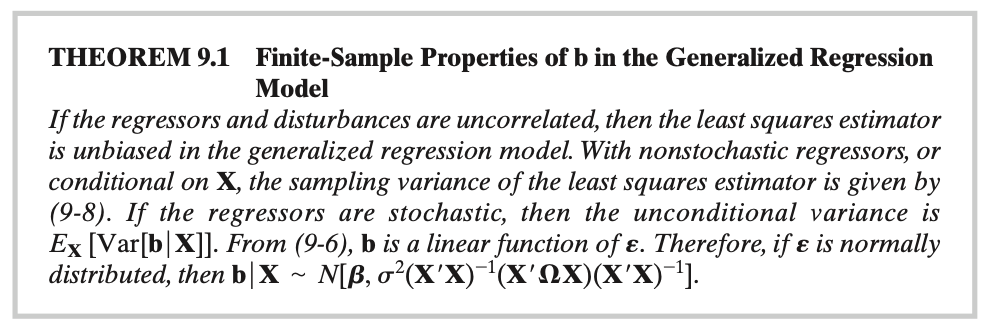
\includegraphics{theorem_9.1.png}
\end{frame}

\begin{frame}{Asymptotic Properties of the Least Squares}
\protect\hypertarget{asymptotic-properties-of-the-least-squares}{}
In the heteroskedastic case, if the variances of \(\varepsilon_i\) are
finite and are not dominated by a single term, so that the conditions of
the Lindeberg-Feller CLT applies, then the LS estimator is
asymptotically normally distributed with covariance matrix

\[Asy.Var[\mathbf{b}]=\frac{1}{n}\mathbf{Q}^{-1}\left[\text{plim }\frac{1}{n}\sum_{i=1}^n{\sigma_i^2\mathbf{x}_i\mathbf{x}_i'}\right]\mathbf{Q}^{-1}\]

\vfill

For the most general case, asymptotic normality is much more difficult
to establish because we might not necessarily have sums of independent
or even uncorrelated random variables.

\vfill

Nonetheless, Amemiya (1985) and Anderson (1971) have established the
asymptotic normality of \(\mathbf{b}\) in a model of autocorrelated
disturbances general enough to include most of the settings we are
likely to meet in practice.

\vfill
\end{frame}

\begin{frame}{Asymptotic Properties of the Least Squares}
\protect\hypertarget{asymptotic-properties-of-the-least-squares-1}{}
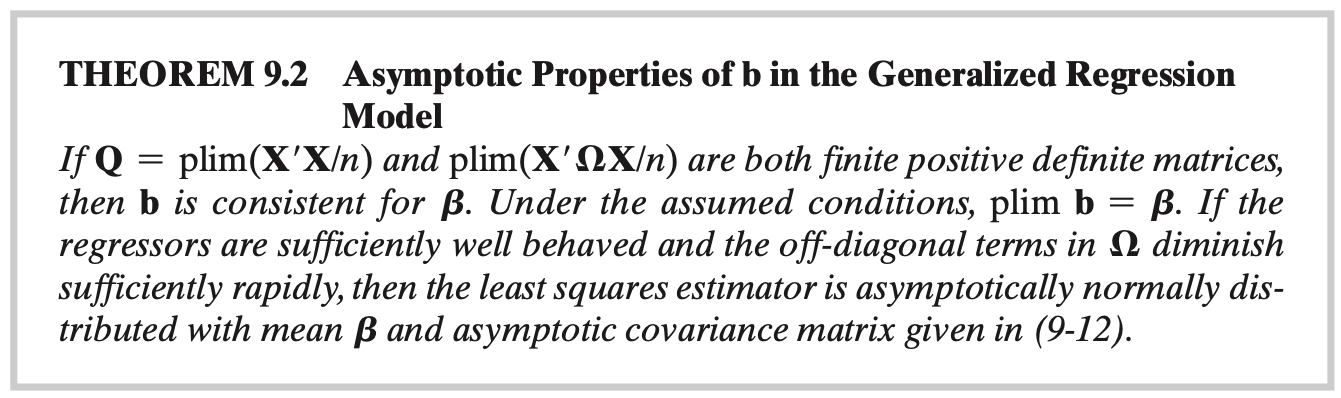
\includegraphics{theorem_9.2.png}
\end{frame}

\begin{frame}{Heteroskedasticity and \(Var[\mathbf{b}|\mathbf{X}]\)}
\protect\hypertarget{heteroskedasticity-and-varmathbfbmathbfx}{}
We have that, for well-behaved regressors,

\[Asy.Var[\mathbf{b}|\mathbf{X}]=\frac{\sigma^2}{n}\mathbf{Q}^{-1}\left(\text{plim }\sum_{i=1}^n{\omega_i\mathbf{x}_i\mathbf{x}_i'} \right)\mathbf{Q}^{-1}\]

In general, we have

\[\mathbf{b} \sim_a N[\mathbf{\beta}, \frac{\sigma^2}{n}\mathbf{Q}^{-1}\mathbf{Q}^*\mathbf{Q}^{-1}], \text{ with }  \mathbf{Q}^*=\text{plim }\sum_{i=1}^n{\omega_i\mathbf{x}_i\mathbf{x}_i'} \]

\vfill

The conventionally estimated covariance matrix for the LS estimator,
however, is \(\sigma^2 (\mathbf{X'X})^{-1}\), which is inappropriate.

\vfill

The appropriate matrix is
\(\sigma^2(\mathbf{X'X})^{-1}(\mathbf{X'\Omega X})(\mathbf{X'X})^{-1}\)

\vfill
\end{frame}

\begin{frame}{Heteroskedasticity and \(Var[\mathbf{b}|\mathbf{X}]\)}
\protect\hypertarget{heteroskedasticity-and-varmathbfbmathbfx-1}{}
We now consider how erroneous the conventional estimator is likely to
be. The difference is

\[Est.Var[\mathbf{b}|\mathbf{X}]-Var[\mathbf{b}|\mathbf{X}]=s^2(\mathbf{X'X})^{-1}-\sigma^2(\mathbf{X'X})^{-1}(\mathbf{X'\Omega X})(\mathbf{X'X})^{-1}\]
In large samples, where \(s^2 \approx \sigma^2\), the difference is
approximately equal to

\[\mathbf{D}=\frac{\sigma^2}{n}\left(\frac{\mathbf{X'X}}{n}\right)^{-1}\left[\frac{\mathbf{X'X}}{n}- \frac{\mathbf{X'}\mathbf{\Omega}\mathbf{X}}{n}\right]\left(\frac{\mathbf{X'X}}{n}\right)^{-1}\]
\end{frame}

\begin{frame}{Heteroskedasticity and \(Var[\mathbf{b}|\mathbf{X}]\)}
\protect\hypertarget{heteroskedasticity-and-varmathbfbmathbfx-2}{}
The difference between the two matrices hinges on the bracketed matrix,

\[\mathbf{\Delta}=\sum_{i=1}^n{(1/n)\mathbf{x}_i\mathbf{x}_i'}-\sum_{i=1}^n{(\omega_i/n)\mathbf{x}_i\mathbf{x}_i'}=\frac{1}{n}\sum_{i=1}^n{(1-\omega_i)\mathbf{x}_i\mathbf{x}_i'}\]

These are two weighted averages of the matrices
\(\mathbf{x}_i\mathbf{x}_i'\) using weights 1 for the first term and
\(\omega_i\) for the second.

\vfill
\end{frame}

\hypertarget{efficient-estimation-by-generalized-least-squares-gls}{%
\subsection{Efficient Estimation by Generalized Least Squares
(GLS)}\label{efficient-estimation-by-generalized-least-squares-gls}}

\begin{frame}{Efficient Estimation by Generalized Least Squares (GLS)}
Efficient estimation of \(\mathbf{\beta}\) in the generalized regression
model requires knowledge of \(\mathbf{\Omega}\).

\vfill

Let's consider the case in which \(\mathbf{\Omega}\) is a known,
symmetric, positive definite matrix.

\vfill

Because \(\mathbf{\Omega}\) is a positive definite symmetric matrix, if
can be factored into

\[\mathbf{\Omega}=\mathbf{C\Lambda C'},\]

where the columns of \(\mathbf{C}\) are the characteristic vectors of
\(\mathbf{\Omega}\) and the characteristic roots of \(\mathbf{\Omega}\)
are arrayed n the diagonal matrix \(\Lambda\).

\vfill
\end{frame}

\begin{frame}{Generalized Least Squares (GLS)}
\protect\hypertarget{generalized-least-squares-gls}{}
Define \(\mathbf{\Lambda}^{1/2}\) as the diagonal matrix with the
\(i\)th diagonal element \(\sqrt{\lambda_i}\) and let
\(\mathbf{T}=\mathbf{C\Lambda^{1/2}}\). Then,

\[\mathbf{TT'}=\mathbf{\Omega}\]

Also let \(\mathbf{P}'=\mathbf{C\Lambda^{-1/2}}\), so
\(\mathbf{\Omega}^{-1}=\mathbf{P'P}\)

\vfill

If we pre-multiply \(\mathbf{y}=\mathbf{X\beta}+\mathbf{\varepsilon}\)
by \(P\), we obtain

\[\mathbf{Py}=\mathbf{PX\beta}+\mathbf{P\varepsilon}\]
\[\mathbf{y_*}=\mathbf{X_*\beta}+\mathbf{\varepsilon_*}\] \vfill
\end{frame}

\begin{frame}{Generalized Least Squares (GLS)}
\protect\hypertarget{generalized-least-squares-gls-1}{}
The conditional variance of \(\mathbf{\varepsilon_*}\) is

\[E[\mathbf{\varepsilon_*}\mathbf{\varepsilon_*}'|\mathbf{X}]=E[\mathbf{P\varepsilon\varepsilon'P'}|\mathbf{PX}]=\mathbf{P}\sigma^2\mathbf{\Omega P'}=\sigma^2\mathbf{I}\]
so the classical regression model applies to the transformed model.

\vfill

Since it is assumed that \(\mathbf{\Omega}\) is known, we can define

\[\begin{split} \hat{\mathbf{\beta}} & =  (\mathbf{X_*'X_*})^{-1}\mathbf{X_*}'\mathbf{y}_* \\
& = (\mathbf{X'P'PX})^{-1}\mathbf{X'P'Py}  \\
& = (\mathbf{X'\Omega^{-1}X})^{-1}\mathbf{X'\Omega^{-1}y}\end{split} \]

We have that \(\hat{\mathbf{\beta}}\) is the efficient estimator of
\(\mathbf{\beta}\) and it is called the Generalized Least Squares (GLS)

\vfill

This is in contrast to the OLS estimator, which uses \(\mathbf{I}\) as
the weighting matrix instead of \(\mathbf{\Omega}^{-1}\).

\vfill

What can we say about the properties of the GLS estimator compared to
the OLS?

\vfill
\end{frame}

\begin{frame}{Properties of the Generalized Least Squares}
\protect\hypertarget{properties-of-the-generalized-least-squares}{}
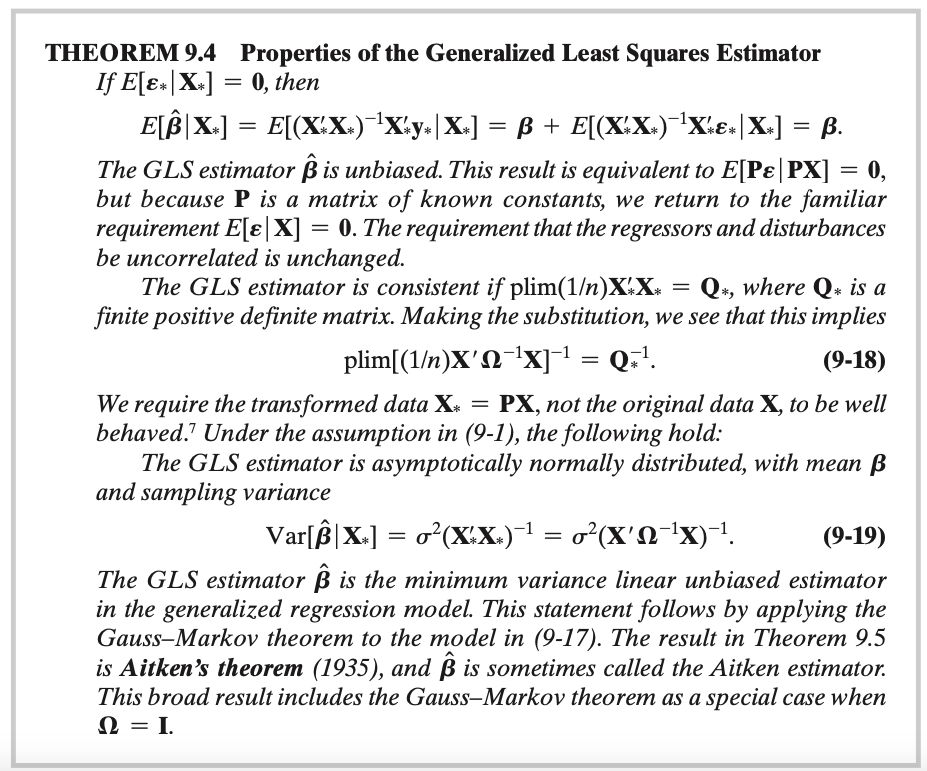
\includegraphics{theorem_9.4.png}
\end{frame}

\begin{frame}{Hypothesis Testing}
\protect\hypertarget{hypothesis-testing}{}
To test hypotheses, we can apply the full set of results we obtained
before to this transformed model.

\vfill

Important to notice, however, that there is no precise counterpart to
the \(R^2\) in the generalized regression model.

\vfill

The GLS estimator minimizes the generalized sum of squares,
\(\varepsilon_*\). There is no assurance that dropping/adding variables
would result in changes in the \(R^2\) based on
\(\hat{\mathbf{\beta}}\).

\vfill
\end{frame}

\begin{frame}{Feasible Generalized Least Squares}
\protect\hypertarget{feasible-generalized-least-squares}{}
To use the results established above, \(\mathbf{\Omega}\) must be known.

\vfill

If \(\mathbf{\Omega}\) contains unknown parameters that need to be
estimated, the GLS is not \textbf{feasible}.

\vfill

But with unrestricted \(\mathbf{\Omega}\), there are far too many
parameters to estimate with \(n\) observations.

\vfill

The typical problem involves a small set of parameters
\(\mathbf{\alpha}\) such that
\(\mathbf{\Omega}=\mathbf{\Omega}(\alpha)\)

\vfill
\end{frame}

\begin{frame}{Feasible Generalized Least Squares}
\protect\hypertarget{feasible-generalized-least-squares-1}{}
A simple heteroskedasticity model would be

\[\sigma^2_i=\sigma^2 z_i^\theta\] for some exogenous variable \(z\).

Suppose that \(\hat{\alpha}\) is a consistent estimator of \(\alpha\).
To make GLS feasible, we shall use
\(\hat{\mathbf{\Omega}}=\mathbf{\Omega}(\hat{\alpha})\)

\vfill

The FGLS estimator is

\[\hat{\hat{\mathbf{\beta}}}= (\mathbf{X'\hat{\Omega}^{-1}X})^{-1}\mathbf{X'\hat{\Omega}^{-1}y}\]

Under some conditions, \(\hat{\hat{\mathbf{\beta}}}\) is asymptotically
equivalent to \(\hat{\mathbf{\beta}}\) and the FGLS estimator based on
\(\hat{\alpha}\) has the same \textbf{asymptotic} properties as the GLS
estimator.

\vfill
\end{frame}

\hypertarget{heteroskedasticity-and-the-weighted-least-squares}{%
\subsection{Heteroskedasticity and the Weighted Least
Squares}\label{heteroskedasticity-and-the-weighted-least-squares}}

\begin{frame}{Heteroskedasticity and the Weighted Least Squares}
The GLS estimator is

\[\hat{\mathbf{\beta}}=(\mathbf{X'\Omega^{-1}X})^{-1}\mathbf{X'\Omega^{-1}y}\]

\(\mathbf{\Omega}^{-1}\) is a diagonal matrix whose \(i\)th diagonal
element is \(1/\omega_i\).

\vfill

The GLS estimator is obtained by regression

\[\mathbf{Py}=\begin{bmatrix}
y_1/\sqrt{\omega_1} \\
y_2/\sqrt{\omega_2} \\
\vdots \\
y_n/\sqrt{\omega_n} \\
\end{bmatrix} \text{ on  } \mathbf{PX}=\begin{bmatrix}
\mathbf{x}'_1/\sqrt{\omega_1} \\
\mathbf{x}'_2/\sqrt{\omega_2} \\
\vdots \\
\mathbf{x}'_n/\sqrt{\omega_n} \\
\end{bmatrix}\]
\end{frame}

\begin{frame}{Heteroskedasticity and the Weighted Least Squares}
\protect\hypertarget{heteroskedasticity-and-the-weighted-least-squares-1}{}
Applying OLS to the transformed model, we obtain the \textbf{weighted
least squares} estimator (WLS)

\[\hat{\mathbf{\beta}}=\left[\sum_{i=1}^n{(1/\omega_i)\mathbf{x}_i\mathbf{x}_i'}\right]^{-1}\left[\sum_{i=1}^n{(1/\omega_i)\mathbf{x}_i\mathbf{y}_i} \right]\]

The logic of the computation is that observations with smaller variances
receive a larger weight in the computations of the sums and therefore
have greater influence in the estimates obtained.

\vfill
\end{frame}

\begin{frame}{Weighted Least Squares with \emph{known}
\(\mathbf{\Omega}\)}
\protect\hypertarget{weighted-least-squares-with-known-mathbfomega}{}
A common specification is that the variance is proportional to the one
of the regressors or its square.

\begin{itemize}
\tightlist
\item
  For example, in a regression of family expenditures, the relevant
  variable is usually income.
\end{itemize}

\vfill

If we assume \(\sigma_i^2=\sigma^2x_{ik}^2,\)

the transformed regression model for GLS is

\[\frac{\mathbf{y}}{\mathbf{x}_k}=\beta_k+\beta_1 \frac{\mathbf{x}_1}{\mathbf{x}_k}+\beta_2 \frac{\mathbf{x}_2}{\mathbf{x}_k}+\ldots++\beta_1 \frac{\mathbf{\varepsilon}}{\mathbf{x}_k}\]

\vfill
\end{frame}

\begin{frame}{Weighted Least Squares with \emph{known}
\(\mathbf{\Omega}\)}
\protect\hypertarget{weighted-least-squares-with-known-mathbfomega-1}{}
If we know the structure of the disturbances variance, we can recover
efficiency by adjusting the data to incorporate this information.

\vfill

However, it is rarely possible to be certain about the nature of the
heteroskedasticity in a regression model.

\vfill

Using the wrong set of weights has two important consequences:

\begin{enumerate}
\tightlist
\item
  WLS becomes inefficient
\item
  the standard errors will be incorrect
\end{enumerate}

\vfill

The standard approach in the literature is to use OLS with the White
estimator or some variant for the asymptotic covariance matrix.

\vfill

Using the wrong
\end{frame}

\hypertarget{testing-for-heteroskdasticity}{%
\subsection{Testing for
Heteroskdasticity}\label{testing-for-heteroskdasticity}}

\begin{frame}{Testing for Heteroskdasticity}
Tests for heteroskedasticity will, in general, be applied to the OLS
residuals (why?)

\vfill

The LS estimator of \(\mathbf{\beta}\), in the presence of
heteroskedasticity, although inefficient, is consistent.

\vfill

Thus, statistics computed using the LS residuals
\(e_i=(y_i-\mathbf{x}_i'\mathbf{b})\) will have the same asymptotic
properties as those computed using the true disturbances
\(\mathbf{\varepsilon}=(y_i-\mathbf{x}_i'\mathbf{\beta})\).

\vfill
\end{frame}

\begin{frame}{White's General Test}
\protect\hypertarget{whites-general-test}{}
White (1960) proposes a general hypothesis of the form

\[\begin{split}
H_0: & \sigma_i^2=E[\varepsilon_i^2|\mathbf{X}]=\sigma^2 \text{ for all } i \\
H_1: & \text{Not } H_0\end{split}\]

An approach is to use an \(F\) test to test the hypothesis that
\(\gamma_1=0\) and \(\gamma_2=0\) in the regression

\[e_i^2=\gamma_0 + \mathbf{X}_i'\mathbf{\gamma}_1+(\mathbf{x}_i\times \mathbf{x}_i')\mathbf{\gamma}_2+\nu_i\]

This test is extremely general. To carry it out, we need not make any
specific assumptions about the nature of the heteroskedasticity.

\vfill
\end{frame}

\begin{frame}{The Breusch-Pagan Test}
\protect\hypertarget{the-breusch-pagan-test}{}
The Breusch-Pagan Test considers \(E[\varepsilon^2|\mathbf{X}]\) to be a
linear function of the explanatory variables:

\[E[\varepsilon^2|\mathbf{X}]=\delta_0 + \delta_1x_1+\ldots+\delta_kx_k+\nu\]
Therefore, the null hypothesis of homoskedasticity is

\[\begin{split}
H_0: & \delta_1=\delta_2=\ldots = \delta_k =0 \\
H_1: & \text{At least of } \delta_j \text{ is not equal to 0}\end{split}\]

Assuming the classical assumptions, \(H_0\) can be tested using the
usual \(F\) test for the joint significance of all explanatory
variables.

\vfill

Notice that we are relying on large sample properties since
\(\varepsilon\geq 0\) cannot be normally distributed.

\vfill
\end{frame}

\begin{frame}{The Breusch-Pagan Test}
\protect\hypertarget{the-breusch-pagan-test-1}{}
The equation we estimate is

\[e_i^2=\delta_0 + \delta_1x_{1i}+\ldots+\delta_kx_{ki}+\varepsilon'_i\]

The steps in performing the test are the following:

\begin{enumerate}
\tightlist
\item
  Estimate \(\mathbf{y}=\mathbf{x\beta}+\varepsilon\) and find \(e\)
\item
  Estimate \(\mathbf{e'e}=\mathbf{x\delta}+\varepsilon'\)
\item
  Perform the \(F\) test for \(\mathbf{\delta}=0\)
\end{enumerate}

\vfill
\end{frame}


\section[]{}
\frame{\small \frametitle{Table of Contents}
\tableofcontents}
\end{document}
